\section{Preliminaries and Notation}
\label{sec:notation}


\begin{defn}
  A \textit{weighted automaton} over a field $\K$ and an alphabet $A$ is a triple 
  $(X,o,t)$ such that $X$ is a finite set of states, 
  $t = \left\lbrace t_a : X \to \K^X\right\rbrace_{a \in A}$
  is a set of transition functions indexed over the symbols of the alphabet $A$ and 
  $o : X  \to \K$ is the output function. 
  The transition functions will be represented as $X \times X$ matrices.
  $A^*$ is the set of all words over $A$, more precisely the free monoid
  with string concatenation as the monoid operation and the empty word $\epsilon$ 
  as the identity element. We denote with $aw$ the
  concatenation of a symbol $a$ to the word $w \in A^*$.
  A weighted language is a function $\psi: A^* \to \K$.
  A function mapping each state vector into its 
  accepted language, $\sqmap{\cdot}: \K^X \to \K^{A^*}$ is defined as follows for 
  every weighted automaton:

  \begin{equation*}
    \begin{aligned}
      \forall v \in \K^X, a \in A, w \in A^* \quad \quad
      \sqmap{v}(\epsilon) = o(v) \quad \quad
      \sqmap{v}(aw) = \sqmap{t_a(v)}(w)  
    \end{aligned}
  \end{equation*}
\end{defn}

Two vectors $v_1, v_2 \in \K^{X\times 1}$ are called weighted language equivalent, 
denoted with  $v_1 \sim_l v_2 $ if and only if 
$ \sqmap {v_1} = \sqmap{v_2}$. One can extend the notion of language 
equivalence to states rather than vectors by assigning 
to each state $x \in X$ the corresponding  unit vector 
$e_x \in \K^X$. When given an initial state $i$ for a weighted automaton, 
the language  of the automaton can be defined as $\sqmap{i}$.


\begin{defn}
  A binary relation $R \subseteq X \times Y$ between two sets $X, Y$ is a 
  subset of the 
  cartesian product of the sets. A relation is called \textit{homogeneous} 
  or an \textit
  {endorelation} if it is a binary relation over $X$ and itself: 
  $R \subseteq X \times
   X$. 
  In such case, it is simply called a binary relation over $X$.
  An \textit{equivalence relation} is a binary relation that is reflexive, 
  symmetric and
  transitive. 
  An equivalence relation which is compatible with all the operations of
the algebraic structure on which it is defined on, is called a 
\textit{congruence relation}. Compatibility with the algebraic structure operations
means that algebraic operations applied on equivalent elements will still
yield equivalent elements. 

\end{defn}



\begin{defn}
  The congruence closure $c(R)$ of a relation R is the smallest congruence relation 
  $R'$ such that $R \subseteq R'$ 
\end{defn}

\begin{defn}
  \label{def:congclos}
  \textit{Generating set for the congruence closure:} \\
  Let $\K$ be a field, $X$ a finite set and $R \subseteq \K^X \times \K^X$
  a relation. Let $(v, v') \in \K^X \times \K^X$ be a pair of vectors.
  The generating set is defined as  $U_R = \left\lbrace u - u' \mid (u, u') \in R \right\rbrace$.
  Then $(v, v') \in c(R) \iff (v - v') \in U_R$
\end{defn}



%===================================================================================

We omit the coalgebraic definition for \textit{linear weighted automata} seen in 
\cite{BONCHI201277} and give a more intuitive definition, which fits our  
implementation when $\K = \R$.
In this implementation, we focus only on weighted automata defined over 
the field of real numbers $\R$. 

\begin{defn}
  A \textit{linear weighted automaton} (in short, LWA) over the field $\K$ and 
  an alphabet $A$
  is a triple  $L = (V, o, \left\lbrace t_a \right\rbrace_{a \in A})$ 
  where $V$ is a vector space representing the state space, and $\dim{(V)} = n$;
  We have that
  $o: V \to \K$ is a linear map associating to each state its output weight,
  and $t = \left\lbrace t_a \in \K^{n \times n} \right\rbrace_{a \in A}$ is
  the set of transition functions, represented with liner maps 
  that for each input $a \in A$ associate the next state, in this case a vector
  in $V$.
  As seen in \cite{boreale2009weighted}, we have that $\dim{(L)} = \dim{(V)} = n$.
\end{defn}

Given a weighted automaton, one can build a corresponding linear weighted automaton
by considering the free vector space generated by the set of states $X$ in the WA,
and by linearizing $o$ and $t$. If $X$ is finite we can use the same matrices for 
$t$ and $o$ in both the WA and the corresponding LWA.
We are only considering a finite number of states and therefore finite dimensional
vector spaces. Let $n$ be the number of states in an WA.
We have that in the corresponding LWA, the transition functions $t_a$ are still
 represented as
$\K^{n \times n}$ matrices. $o \in \K^{1 \times n}$ is represented as a row vector.
$t_a(v)$ denotes the vector obtained by multiplying the matrix $t_a$ by the column 
vector $v  \in \K^{n \times 1}$. $o(v)$ denotes the scalar $s \in \K$ obtained by 
dot product of the row vector $o$ with $v \in \K^{n \times 1}$.

\begin{defn}
  The language recognized by a vector $v \in V$ in an LWA $(V,o,t)$ is defined
  for all words $w \in A*$ as $\langlwa{v}{V}(w) = o(v_n)$ where $v_n$ is the 
  vector reached from $v$ through the composition of the transition functions
  corresponding to each symbol in $w$.
  
  \begin{equation*}
    \begin{aligned}
      \langlwa{v}{V}(w) = \begin{cases}
        o(v) & \text{if } w = \epsilon \\ 
        \langlwa{t_a(v)}{V}(w') & \text{if } w = aw' 
      \end{cases}
    \end{aligned}
  \end{equation*}
  
\end{defn}


We define the equivalence relation  $\llwb$ for a given LWA $L = (V, o, t)$ as 

\begin{equation}
  \forall v_1, v_2 \in V, \; v_1 \llwb v_2 \iff \langlwa{v_1}{V} = \langlwa{v_2}{V}
\end{equation}

Proofs are available in section 3.3 of \cite{BONCHI201277}

Language equivalence can be now expressed in terms of linear weighted 
bisimulations (LWBs for short).
Differently from weighted bisimulations, LWBs can be seen both as relations 
and as subspaces.
The subspace representation of LWBs is used in the backwards partition 
refinement algorithm 
implemented in \cite{BONCHI201277} and in this work.

\begin{defn}
  \label{def:linrel}
  \textit{Linear Relations:}\\
  Let $U$ be a subspace of $V$. The binary relation $R_U$ over $V$ is defined by
  \begin{equation*}
    \begin{aligned}
      v_1 \; R_U \; v_2 \quad \iff \quad v_1 - v_2 \in U
    \end{aligned}
  \end{equation*}
  The relation $R$ is linear if there exists a subspace $U$ such that $R = R_U$.
  A linear relation is a total equivalence relation on $V$.
\end{defn}

\begin{defn}
  \textit{Kernel of a Relation and Linear Extension} \\
  Let $R$ be a binary relation over V. 
  The \textit{kernel} of $R$, is the set 
  $\mker{R} = \left\lbrace v_1 - v_2 \mid v_1 \; R \; v_2 \right\rbrace$.
  The \textit{linear extension} of $R$, written as $R^\ell$, is defined by 
  \begin{equation*}
    \begin{aligned}
      v_1 \; R^\ell \; v_2  \quad \iff \quad (v_1 - v_2) \in \mspan{\mker{R}}
    \end{aligned}
  \end{equation*}
\end{defn}

\begin{lem}
  Let $U$ be a subspace of $V$, then $\mker{R_U} = U$
\end{lem}

\begin{defn}
  \textit{Linear Weighted Bisimulation:} \\
  Let $(V, o, t)$ be a linear weighted automaton. A linear relation 
  $R \subseteq V \times V$ is a \textit{linear weighted bisimulation} if 
  $\forall (v_1, v_2) \in R$ it holds that: 
  \begin{center}
    \begin{enumerate}
      \item $o(v_1) = o(v_2)$
      \item $\forall a \in A, \; t_a(v_1) \; R \; t_a(v_2)$
    \end{enumerate}
  \end{center}
\end{defn}

\begin{lem}
  Let $(V, o, t)$ be a linear weighted automaton. A linear relation 
  $R$ over $V$ is a linear weighted bisimulation if and only if
\end{lem}
  \begin{center}
    \begin{enumerate}
      \item $R \subseteq \mker{o}$
      \item $R$ is $t_a$-invariant $\forall a \in A$
    \end{enumerate}
  \end{center}

Theorem 3 in section 3.3 of \cite{BONCHI201277}, states that 
$\mker{\langlwa{-}{V}}$ is the largest linear weighted bisimulation on $V$.
As a corollary, we obtain that $\llwb$ is the largest linear weighted bisimulation.

We now introduce a lemma that will be fundamental in the next sections of this work.

\begin{lem}
  \label{lem:coincide}
  $\llwb$ coincides with $\sim_l$: 

  %Let $(X, o, t)$ be a WA and $(\K^X, o^\sharp, t^\sharp)$ the corresponding linear 
  %weighted automaton. Then $\forall x \in X, \;\; \sqmap{x} = \langlwa{x}{\K^X}$
\end{lem}

\begin{figure}[htbp!]
  \centering
  

\tikzset{every picture/.style={line width=0.75pt}} %set default line width to 0.75pt        

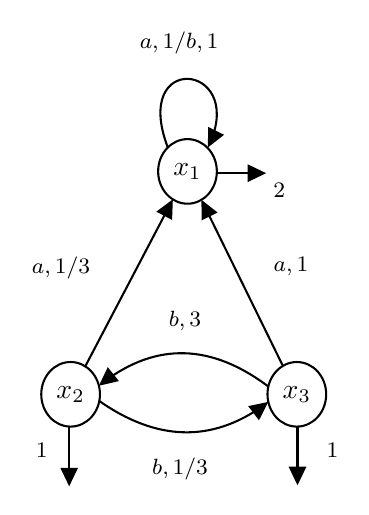
\begin{tikzpicture}[x=0.75pt,y=0.75pt,yscale=-1,xscale=1]
%uncomment if require: \path (0,514); %set diagram left start at 0, and has height of 514

%Curve Lines [id:da7520674866212254] 
\draw    (207.69,98.63) .. controls (223.51,60.79) and (169.45,55.3) .. (187,101.61) ;
\draw [shift={(206.33,101.61)}, rotate = 296.28] [fill={rgb, 255:red, 0; green, 0; blue, 0 }  ][line width=0.08]  [draw opacity=0] (8.93,-4.29) -- (0,0) -- (8.93,4.29) -- cycle    ;
%Straight Lines [id:da36516510379788225] 
\draw    (139.5,236.5) -- (139.5,261.86) ;
\draw [shift={(139.5,264.86)}, rotate = 270] [fill={rgb, 255:red, 0; green, 0; blue, 0 }  ][line width=0.08]  [draw opacity=0] (8.93,-4.29) -- (0,0) -- (8.93,4.29) -- cycle    ;
%Straight Lines [id:da06517112562563687] 
\draw    (249.5,236) -- (249.5,261.36) ;
\draw [shift={(249.5,264.36)}, rotate = 270] [fill={rgb, 255:red, 0; green, 0; blue, 0 }  ][line width=0.08]  [draw opacity=0] (8.93,-4.29) -- (0,0) -- (8.93,4.29) -- cycle    ;
%Straight Lines [id:da05488487732501923] 
\draw    (211,114) -- (231.4,114) ;
\draw [shift={(234.4,114)}, rotate = 180] [fill={rgb, 255:red, 0; green, 0; blue, 0 }  ][line width=0.08]  [draw opacity=0] (8.93,-4.29) -- (0,0) -- (8.93,4.29) -- cycle    ;

% Text Node
\draw    (196.5, 113.15) circle [x radius= 14.14, y radius= 15.56]   ;
\draw (196.5,113.15) node  [font=\normalsize]  {$x_{1}$};
% Text Node
\draw    (140.18, 220.54) circle [x radius= 14.14, y radius= 15.56]   ;
\draw (140.18,220.54) node  [font=\normalsize]  {$x_{2}$};
% Text Node
\draw    (249.18, 220.54) circle [x radius= 14.14, y radius= 15.56]   ;
\draw (249.18,220.54) node  [font=\normalsize]  {$x_{3}$};
% Text Node
\draw (178,249.9) node [anchor=north west][inner sep=0.75pt]  [font=\footnotesize]  {$b,1/3$};
% Text Node
\draw (186,178.9) node [anchor=north west][inner sep=0.75pt]  [font=\footnotesize]  {$b,3$};
% Text Node
\draw (236.5,152.9) node [anchor=north west][inner sep=0.75pt]  [font=\footnotesize]  {$a,1$};
% Text Node
\draw (172,44.4) node [anchor=north west][inner sep=0.75pt]  [font=\footnotesize]  {$a,1/b,1$};
% Text Node
\draw (120,152.9) node [anchor=north west][inner sep=0.75pt]  [font=\footnotesize]  {$a,1/3$};
% Text Node
\draw (122,242.65) node [anchor=north west][inner sep=0.75pt]  [font=\footnotesize]  {$1$};
% Text Node
\draw (262,242.65) node [anchor=north west][inner sep=0.75pt]  [font=\footnotesize]  {$1$};
% Text Node
\draw (236.4,117.4) node [anchor=north west][inner sep=0.75pt]  [font=\footnotesize]  {$2$};
% Connection
\draw    (154.02,223.76) .. controls (181.71,243.14) and (208.08,243.86) .. (233.12,225.93) ;
\draw [shift={(235.43,224.21)}, rotate = 502.59] [fill={rgb, 255:red, 0; green, 0; blue, 0 }  ][line width=0.08]  [draw opacity=0] (8.93,-4.29) -- (0,0) -- (8.93,4.29) -- cycle    ;
% Connection
\draw    (235.45,216.79) .. controls (208,196.14) and (181.57,195.41) .. (156.17,214.59) ;
\draw [shift={(153.82,216.42)}, rotate = 321.14] [fill={rgb, 255:red, 0; green, 0; blue, 0 }  ][line width=0.08]  [draw opacity=0] (8.93,-4.29) -- (0,0) -- (8.93,4.29) -- cycle    ;
% Connection
\draw    (147.25,207.06) -- (188.04,129.28) ;
\draw [shift={(189.43,126.63)}, rotate = 477.67] [fill={rgb, 255:red, 0; green, 0; blue, 0 }  ][line width=0.08]  [draw opacity=0] (8.93,-4.29) -- (0,0) -- (8.93,4.29) -- cycle    ;
% Connection
\draw    (242.46,206.85) -- (204.54,129.53) ;
\draw [shift={(203.22,126.84)}, rotate = 423.87] [fill={rgb, 255:red, 0; green, 0; blue, 0 }  ][line width=0.08]  [draw opacity=0] (8.93,-4.29) -- (0,0) -- (8.93,4.29) -- cycle    ;

\end{tikzpicture}

  \begin{equation*}
    \begin{aligned}
      o = \begin{pmatrix}
        2 & 1 & 1
      \end{pmatrix} & \quad &  
      T_a = \begin{pmatrix}
        1 & \frac{1}{3} & 1 \\ 
        0 & 0 & 0 \\
        0 & 0 & 0 \\ 
      \end{pmatrix} & \quad &
      T_b = \begin{pmatrix}
        1 & 0 & 0 \\ 
        0 & 0 & 3 \\
        0 & \frac{1}{3} & 0 \\ 
      \end{pmatrix} & \quad &
    \end{aligned}
  \end{equation*}
  \caption{Example of a Weighted Automata}
  \label{fig:autexmp}
\end{figure}